\chapter{Đại số cơ bản}

\section{Ánh xạ}

Cho 2 tập hợp $X$ và $Y$. Ánh xạ $f$ biến một phần tử $x \in X$ thành một và chỉ một phần tử $y \in Y$.

Ta ký hiệu
\[f: X \to Y, \; f(x) = y\]

Khi đó, $X$ được gọi là tập nguồn (domain) và $Y$ là tập đích (image).

Ánh xạ có 3 loại:

\begin{itemize}[noitemsep]
    \item Đơn ánh (Injection): Hai phần tử khác nhau của tập nguồn cho hai ảnh khác nhau. Tức là với mọi $x_1, x_2 \in X$ mà $x_1 \neq x_2$, thì $f(x_1) \neq f(x_2)$
    \item Toàn ánh (Surjection): Mọi phần tử $y \in Y$ đều có ít nhất một phần tử $x \in X$ mà $f(x) = y$. Nói cách khác với mỗi phần tử trong $Y$ ta đều tìm được phần tử thuộc $X$ biến thành nó
    \item Song ánh (Injection): Nếu ánh xạ đó vừa là đơn ánh, vừa là toàn ánh
\end{itemize}

\begin{remark}
    Dựa vào định nghĩa và hình vẽ, ta có thể rút ra kết luận như sau
    \begin{itemize}[noitemsep]
        \item Đối với đơn ánh, do mọi phần tử của $X$ đều có ảnh ở $Y$, tuy nhiên có thể có phần tử ở $Y$ không do phần tử nào của $X$ biến thành (trong hình là 5). Do đó $| X | \leq | Y |$
        \item Đối với toàn ánh, mọi phần tử của $Y$ đều có nguồn gốc xuất xứ, tuy nhiên có thể có phần tử của $X$ không biến thành $y$ nào của $Y$ (trong hình là $e$). Do đó $| X | \geq | Y |$
        \item Đối với song ánh, do là kết hợp giữa đơn ánh và toàn ánh, khi đó dấu đẳng thức xảy ra, $| X | = | Y |$
    \end{itemize}
\end{remark}

\begin{figure}[ht]
    \centering
    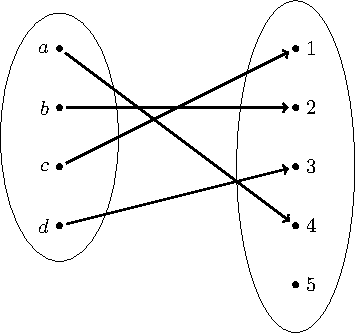
\includegraphics{pics/maps/injection.pdf}
    \caption{Đơn ánh}
\end{figure}

\begin{figure}[ht]
    \centering
    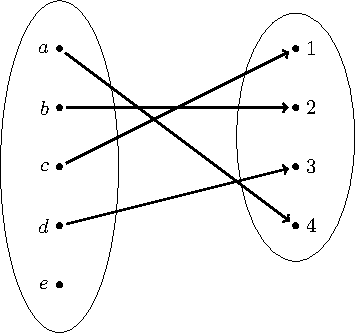
\includegraphics{pics/maps/surjection.pdf}
    \caption{Toàn ánh}
\end{figure}

\begin{figure}[ht]
    \centering
    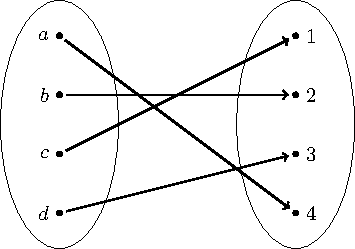
\includegraphics{pics/maps/bijection.pdf}
    \caption{Song ánh}
\end{figure}

\section{Hàm số}

Khi 2 tập nguồn và đích của ánh xạ là 2 tập hợp số, ta có hàm số.

\begin{example}
    Hàm số $f: \RR \rightarrow \RR$ với $y = f(x) = x^3 + x + 1$. Ở đây $X \equiv \RR$ và $Y \equiv \RR$.
\end{example}

Lưu ý rằng tập nguồn và đích không nhất thiết là tập hợp số cơ bản ($\QQ, \RR$) mà cũng có thể là tích Descartes của chúng.

\begin{example}
    Hàm số $f: \RR \times \RR \rightarrow \RR$ với $z = f(x, y) = x + y + xy$. Ở đây $X \equiv \RR$, $Y \equiv \RR$ và $Z \equiv \RR$.
\end{example}

Chúng ta còn một cách gọi khác cho đơn ánh, toàn ánh, song ánh trong tiếng Anh.

\begin{table}[ht]
    \centering
    \begin{tabular}{| l | l | l |}
        \hline
        đơn ánh & injection & one-to-one map \\
        \hline
        toàn ánh & surjection & onto map \\
        \hline
        song ánh & bijection & one-to-one and onto map \\
        \hline
    \end{tabular}

    \caption{Thuật ngữ tiếng Anh cho ánh xạ}
\end{table}

\begin{example}
    Hàm số $f: \RR \rightarrow \RR$ cho bởi $y = f(x) = x^3$ là song ánh.

    \begin{proof}
        Ta thấy nếu $f(x_1) = f(x_2)$, tương đương $x_1^3 = x_2^3$ nên $x_1 = x_2$. Do đó $f$ là đơn ánh.

        Với mọi $y = x^3 \in \RR$, do căn bậc 3 luôn tồn tại nên ta có $x = \sqrt[3]{y}$. Nghĩa là luôn tồn tại $x$ để $f(x) = y$ với mọi $y \in \RR$. Do đó $f$ là toàn ánh.

        Kết luận $f$ là song ánh.
    \end{proof}
\end{example}

\section{Đồng biến và nghịch biến}

\begin{definition}
    Xét hàm số $f(x)$ xác định trên khoảng $(a, b)$. Ta nói $f(x)$ đồng biến (tăng) trên $(a, b)$ 
    nếu với mọi $x_1, x_2 \in (a, b)$ mà $x_1 < x_2$ ta có $f(x_1) < f(x_2)$.
\end{definition}

Tương tự $f(x)$ nghịch biến (giảm) trên $(a, b)$ nếu với mọi $x_1, x_2 \in (a, b)$ mà 
$x_1 < x_2$ ta có $f(x_1) > f(x_2)$.
Lưu ý ở các so sánh trên dấu bằng có thể xảy ra. Khi đó hàm số
được gọi là tăng \textit{không nghiêm ngặt} (hoặc giảm \textit{không
nghiêm ngặt}).

Nếu hàm số đồng biến (hoặc nghịch biến) trên khoảng xác định nào đó thì ta
nói hàm số đơn điệu trên khoảng đó.

Đồ thị của hàm số khi đồng biến sẽ đi lên (theo chiều từ trái sang phải), và đi
xuống nếu nghịch biến.

\begin{example}
    Khảo sát sự biến thiên của hàm số $f(x) = x^2 + 3$.

    Để khảo sát sự biến thiên, một cách làm đơn giản theo định nghĩa
    là ta xét $x_1 < x_2$ và so sánh $f(x_1)$ với $f(x_2)$.

    Ta có $f(x_1) - f(x_2) = x_1^2 + 3 - x_2^2 - 3 = (x_1 - x_2)(x_1 + x_2)$

    Do $x_1 < x_2$, nên với $x_1, x_2 > 0$ thì $x_1 + x_2 > 0$ và
    $x_1 - x_2 < 0$. Suy ra $f(x_1) - f(x_2) < 0$ và từ đó $f(x_1) < f(x_2)$. Như
    vậy $f(x)$ đồng biến trên $(0, +\infty)$.

    Tương tự, khi $x_1, x_2 < 0$ thì $x_1 + x_2 < 0$. Khi đó $f(x_1) > f(x_2)$
    nên $f(x)$ nghịch biến trên $(-\infty, 0)$.
\end{example}

Để thể hiện sự biến thiên của hàm số ta sử dụng bảng biến thiên.
Đối với hàm số $y = x^2 + 3$ ở trên bảng biến thiên có dạng:

\begin{figure}[bh]
    \centering
    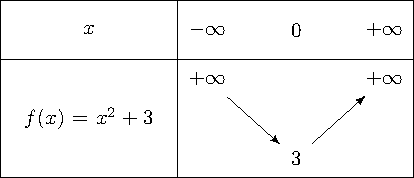
\includegraphics{pics/algebra/algebra1.pdf}
    \caption{Bảng biến thiên hàm số $y=x^2 + 3$}
\end{figure}

Ta đã chứng minh được hàm số nghịch biến trên $(-\infty, 0)$
và đồng biến trên $(0, +\infty)$, giá trị $f(0) = 3$ nên bảng
biến thiên thể hiện sự tăng giảm trên các khoảng. Dựa vào 
bảng biến thiên ta có thể hình dung ra dạng của đồ thị hàm số.

\section{Đồ thị hàm số}

Để biểu diễn sự phụ thuộc của biến $y$ theo biến $x$, hay 
nói cách khác là biểu diễn hàm số $y=f(x)$ ta có thể dùng đồ thị.

Đồ thị được vẽ trên hệ tọa độ Descartes $Oxy$. Bảng biến thiên
cho ta thấy tính đơn điệu trên các khoảng xác định, và đồ thị
sẽ cho ta thấy rõ hơn độ "cong" của những đường cong.

\begin{example}
    Với hàm số $y = x^2 + 3$ ở trên. Đồ thị hàm số có dạng như sau:
    \begin{figure}[bh]
        \centering
        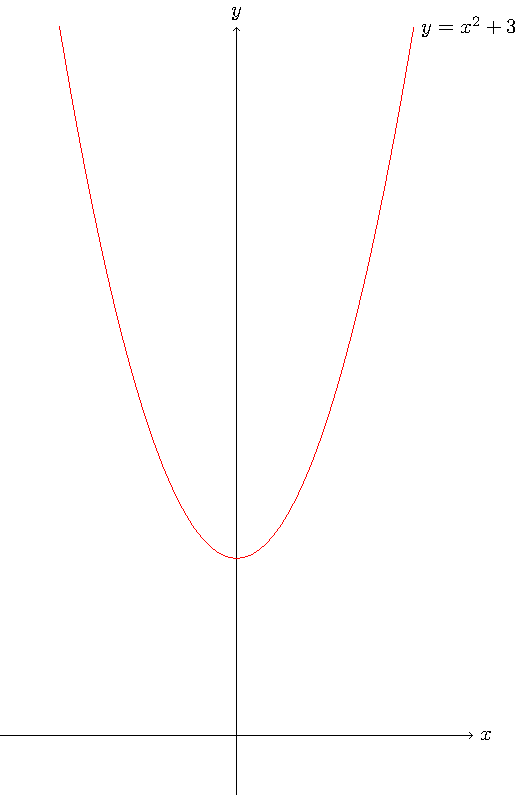
\includegraphics[scale=0.75]{pics/algebra/algebra2.pdf}
        \caption{Đồ thị hàm số $y=x^2 + 3$}
    \end{figure}
\end{example}

\begin{example}
    Với hàm số $y = \dfrac{1}{x}$. Ta thấy rằng hàm số không xác
    định tại $x=0$. Khảo sát sự biến thiên như bên trên ta thấy
    hàm số nghịch biến ở 2 khoảng xác định là $(-\infty, 0)$
    và $(0, +\infty)$. Đồ thị hàm số có dạng như sau:
    \begin{figure}[ht]
        \centering
        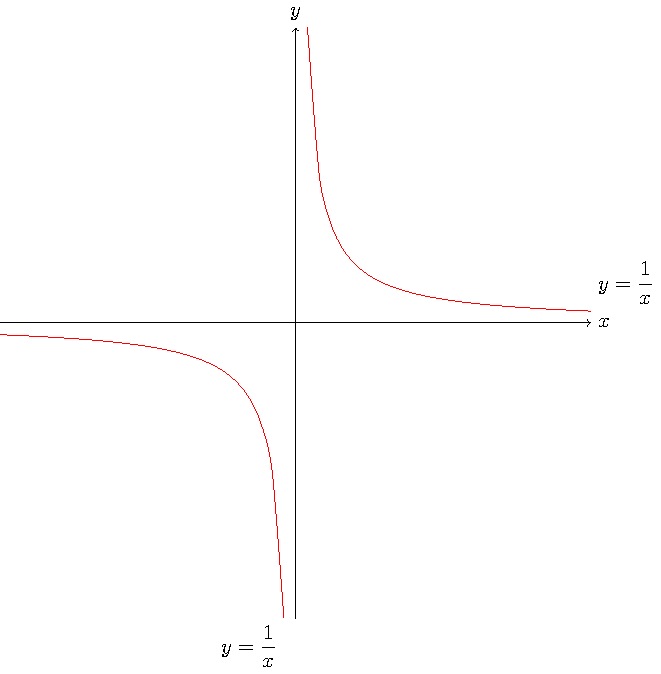
\includegraphics[scale=0.75]{pics/algebra/algebra3.pdf}
        \caption{Đồ thị hàm số $y = \dfrac{1}{x}$}
    \end{figure}
\end{example}

Từ đồ thị của 2 hàm số trên ta thấy rằng mặc dù cùng là nghịch biến
trên $(-\infty, 0)$ nhưng nghịch biến của $y=x^2+3$ nhìn "nhẹ nhàng" hơn. Trong khi 
đồ thị $y = \dfrac{1}{x}$ thì ban đầu "nhẹ nhàng", sau thì như
"rơi tự do".